\chapter{Технологический раздел}

В этом разделе осуществляется выбор инструментов для реализации, предоставляется описание разрабатываемой базы данных и ее структуры, а также приводятся примеры работы программы.

\section{Технологии, используемые при \newline создании ПО}

Для выполнения данной курсовой работы был выбран язык \newline $Python$~\cite{python-lang}.

Для взаимодействия с базами данных в объектно--ориентированной парадигме была выбрана технология $SQLAlchemy$~\cite{sqlalchemy}.

Для работы с базой данных была выбрана СУБД $PostgreSQL$~\cite{postgresql}.

\section{Архитектура ПО}

В процессе разработки были реализованы следующие структуры:
\begin{enumerate}[label=\arabic*)]
    \item Flight --- описывает информацию о полете;
    \item Delay --- описывает информацию о задержке;
    \item Airport --- описывает информацию об аэропорте;
    \item Airline --- описывает информацию об авиакомпании;
    \item Plane --- описывает информацию о самолете;
    \item Crew --- описывает информацию о членах экипажа;
    \item Report --- описывает информацию о отчетах;
    \item System --- описывает информацию о системах;
\end{enumerate}

Также была создана функция, проверяющая наличие необходимой роли у пользователя для выполнения отправленного запроса.

\section{Реализация триггера}

В листинге~\ref{lst:trigger} представлен триггер для обновления данных в таблице system при добавлении нового отчета о самолете в таблицу report.

\begin{lstlisting}[label=lst:trigger, caption=Триггер для обновления данных в таблице system, language=SQL]
def create_trigger(db: Session):
    sql = """
    CREATE OR REPLACE FUNCTION decrease_k_coeff() RETURNS TRIGGER AS $$
    BEGIN
    UPDATE systems
    SET k_coeff = k_coeff - (random() * 10)
    WHERE plane = NEW.plane;
    RETURN NEW;
    END;
    $$ LANGUAGE plpgsql;

    CREATE TRIGGER decrease_k_coeff_trigger
    AFTER INSERT ON reports
    FOR EACH ROW EXECUTE FUNCTION decrease_k_coeff();
    """
    db.execute(text(sql))
\end{lstlisting}

\section{Реализация хранимой процедуры}
В листинге~\ref{lst:procedure} представлена хранимая процедура для получения вероятности задержки рейса.

\begin{lstlisting}[label=lst:procedure, caption=Хранимая процедура для получения вероятности задержки рейса, language=SQL]
CREATE OR REPLACE PROCEDURE probability(
plane VARCHAR,
origin VARCHAR,
destination VARCHAR,
date_limit VARCHAR
)
LANGUAGE plpgsql
AS $$
BEGIN
    CREATE TEMP TABLE IF NOT EXISTS temp_result (
        airport VARCHAR,
        average_delay FLOAT,
        total_delays INT,
        delay_percentage FLOAT
    ) ON COMMIT DROP;

    INSERT INTO temp_result
    SELECT
        dest_airport.display_airport_name AS airport,
        AVG(d.dep_delay) as average_delay,
        COUNT(d.dep_delay) as total_delays,
        ((CAST(COUNT(d.dep_delay) AS FLOAT) /
        (SELECT COUNT(*) FROM flights WHERE tail_num = plane AND fl_date::DATE < date_limit::DATE)) * 100.0) as delay_percentage
    FROM
        flights f
    JOIN
        flight_airport fa_origin ON f.id = fa_origin.flight_id
    JOIN
        airports origin_airport ON fa_origin.airport_id = origin_airport.id AND fa_origin.airport_type = 'departure'
    JOIN
        flight_airport fa_dest ON f.id = fa_dest.flight_id
    JOIN
        airports dest_airport ON fa_dest.airport_id = dest_airport.id AND fa_dest.airport_type = 'arrival'
    JOIN
        delay d ON f.id = d.id
    WHERE
        f.tail_num = plane AND
        origin_airport.airport_code = origin AND
        dest_airport.airport_code = destination AND
        f.fl_date::DATE < date_limit::DATE
    GROUP BY
        dest_airport.display_airport_name;
END;
$$;
\end{lstlisting}

\section{Реализация системы ролей}

В листинге~\ref{lst:roles} представлен код создания ролей в системе, в котором выдаются права на определенные таблицы в базе данных.

\begin{lstlisting}[label=lst:roles, caption=Создание ролей в системе, language=SQL]
CREATE ROLE guest;
CREATE ROLE employee;
CREATE ROLE admin;

GRANT SELECT ON flights, airports, airlines, delay TO guest;

GRANT ALL PRIVILEGES ON reports, systems, checklist TO employee;

GRANT ALL PRIVILEGES ON ALL TABLES IN SCHEMA public TO admin;
\end{lstlisting}

\newpage
\section{Тестирование триггера}
В соответствии со схемой алгоритма триггера, указанной на Рисунке~\ref{fig:trigger}, алгоритм включает проверку наличия уже существующего отчета для самолета Х в таблице reports.
Для целей тестирования, значение, на которое уменьшается коэффициент, было заменено с random() на 10.

В таблице~\ref{tab:tabl10} представлены модульные тесты для триггера базы данных.
\begin{table}[H]
    \centering
    \captionsetup{justification=raggedright}
    \caption{Модульное тестирование триггера базы данных (ч. 1)}
    \begin{tabular}{|c|p{0.3\textwidth}|p{0.3\textwidth}|p{0.2\textwidth}|}
        \hline
        № & Класс \newline эквивалентности & Запрос для теста & Результат \\
        \hline
        1 & Вставка первого \newline отчета для самолета N10156 в таблицу reports с k\_coeff = 100 & INSERT INTO reports (tail\_num, avg\_rate, decision, datetime) VALUES ('N10156', 100, `true', `2024-06-09 00:54:53'); & k\_coeff = 90 \\
        \hline
        2 & Вставка второго \newline отчета для самолета N10156 в таблицу reports с k\_coeff = 90 & INSERT INTO reports (tail\_num, avg\_rate, decision, datetime) VALUES ('N10156', 100, `true', `2024-06-09 01:54:53'); & k\_coeff = 80 \\
        \hline
        3 & Вставка третьего отчета для самолета N10156 в таблицу reports с k\_coeff = 80 & INSERT INTO reports (tail\_num, avg\_rate, decision, datetime) VALUES ('N10156', 100, `true', `2024-06-09 02:54:53'); & k\_coeff = 70 \\
        \hline
    \end{tabular}
    \label{tab:tabl10}
\end{table}


\begin{table}[H]
    \centering
    \captionsetup{justification=raggedright}
    \caption{Модульное тестирование триггера базы данных (ч. 2)}
    \begin{tabular}{|c|p{0.3\textwidth}|p{0.3\textwidth}|p{0.2\textwidth}|}
        \hline
        № & Класс \newline эквивалентности & Запрос для теста & Результат \\
        \hline
        4 & Вставка отчета для \newline самолета N10156 в таблицу reports с \newline k\_coeff = 0 & INSERT INTO reports (tail\_num, avg\_rate, decision, datetime) VALUES ('N10156', 100, `true', `2024-06-09 02:54:53'); & k\_coeff = 0 \\
        \hline
        5 & Вставка отчета для несуществующего самолета в таблицу reports & INSERT INTO reports (tail\_num, avg\_rate, decision, datetime) VALUES ('N10157', 100, `true', `2024-06-09 02:54:53'); & Ошибка: данный самолет не существует \\
        \hline
        6 & Вставка отчета для \newline существующего \newline самолета в таблицу reports с \newline некорректными \newline данными & INSERT INTO reports (tail\_num, avg\_rate, decision, datetime) VALUES ('N10156', 100, `true', `2024-06-09 02:54:53'); & Ошибка: некорректные данные \\
        \hline
    \end{tabular}
    \label{tab:tabl11}
\end{table}

В процессе тестирования были выполнены запросы, указанные в Таблицах~\ref{tab:tabl10}-\ref{tab:tabl11}.
После их выполнения, в случае успешного завершения, проводилась проверка соответствия текущего состояния кортежа ожидаемому, и получалось сообщение, соответствующее таблице.
Если ожидался неудачный исход, проверялось наличие сообщения об ошибке, соответствующего таблице, и состояние кортежа должно было соответствовать его предыдущему состоянию.

\newpage
\section{Примеры работы}
На рисунках~\ref{fig:example_employee},~\ref{fig:example_flight},~\ref{fig:example_probability} представлены примеры работы приложения.

\begin{itemize}
    \item авторизация сотрудника;
    \begin{figure}[H]
        \centering
        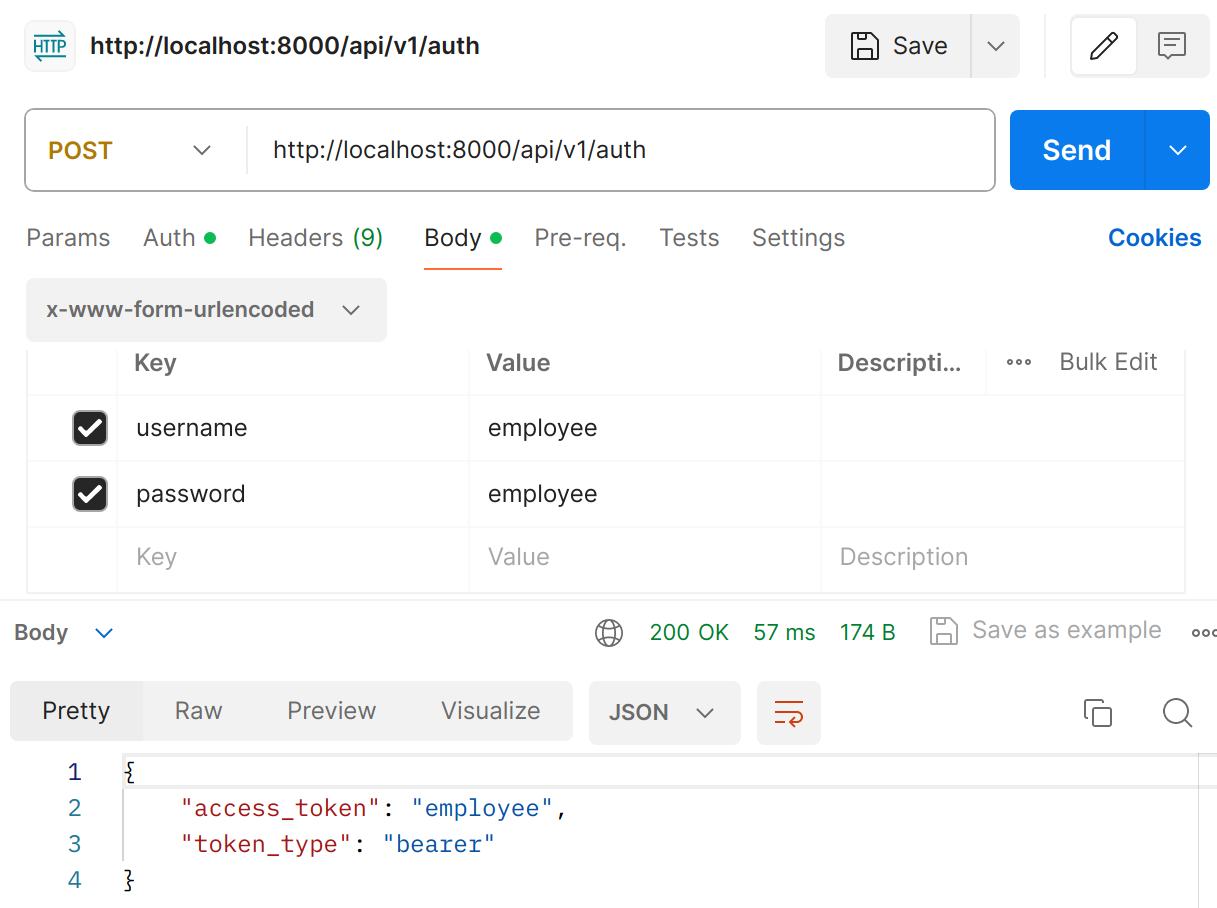
\includegraphics[scale=0.2]{inc/example_employee}
        \caption{Пример работы программы}
        \label{fig:example_employee}
    \end{figure}

    \item получение информации о полете;
    \begin{figure}[H]
              \centering
              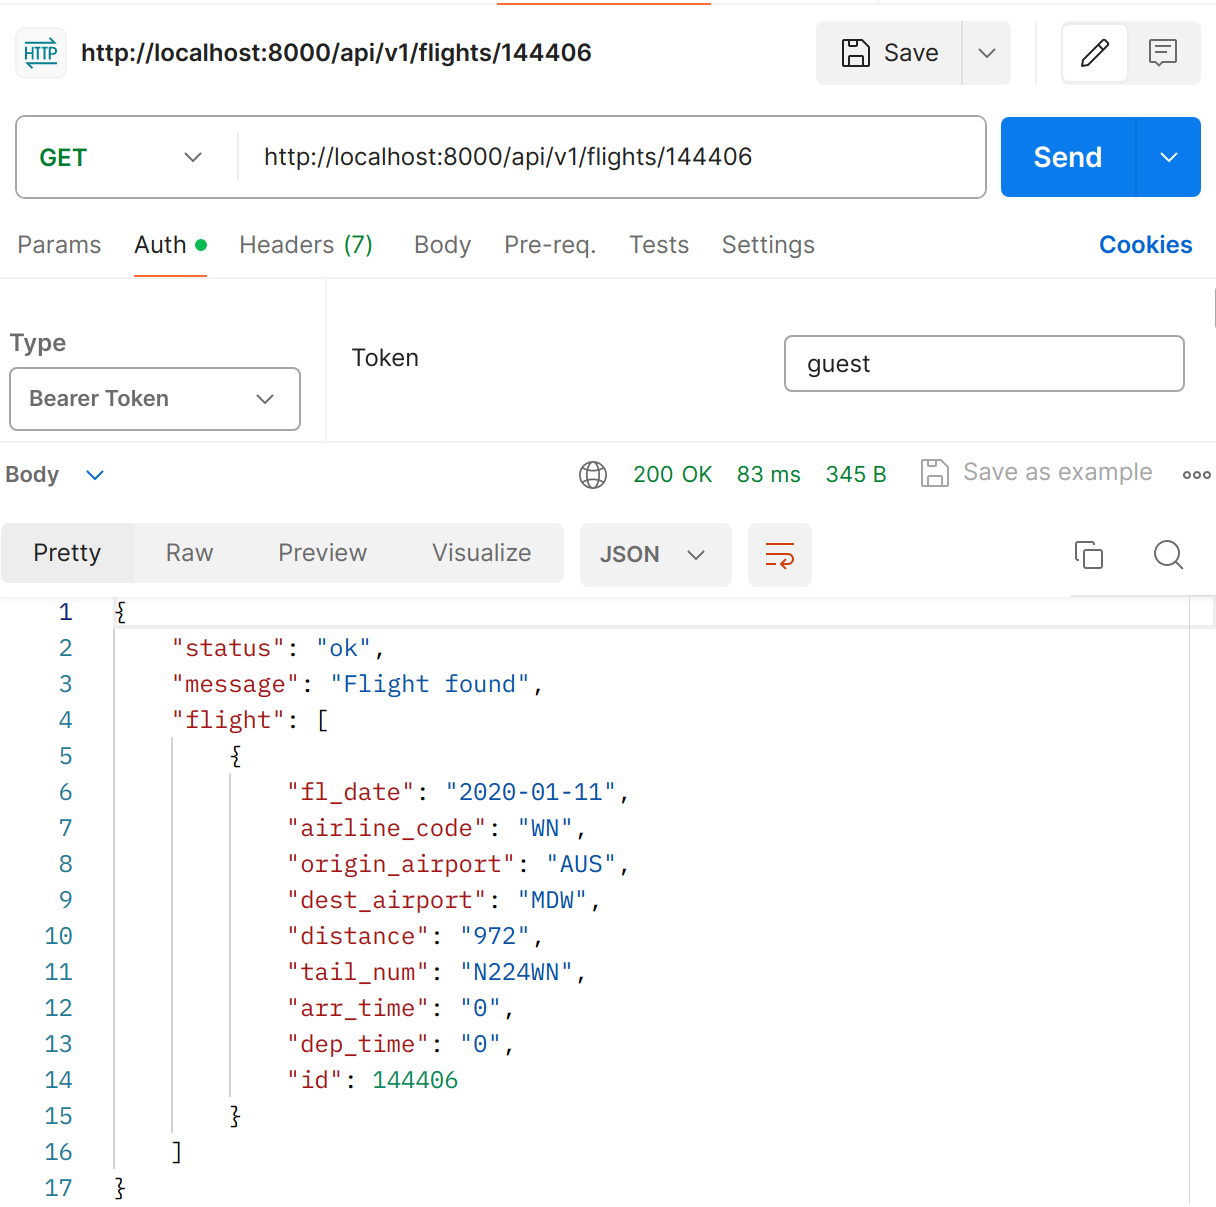
\includegraphics[scale=0.2]{inc/example_flight}
              \caption{Пример работы программы}
              \label{fig:example_flight}
    \end{figure}

    \item получение информации о вероятности задержки полета;
    \begin{figure}[H]
              \centering
              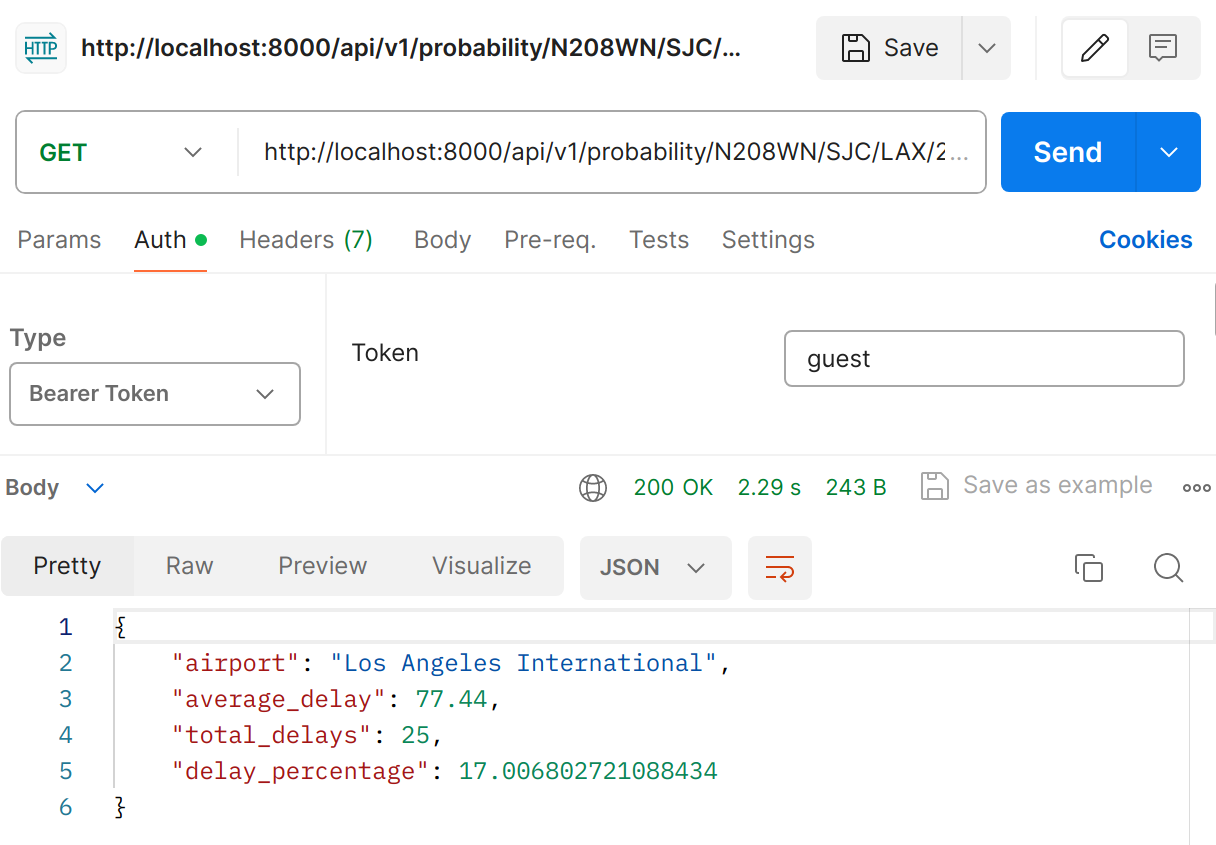
\includegraphics[scale=0.2]{inc/example_probability}
              \caption{Пример работы программы}
              \label{fig:example_probability}
    \end{figure}
\end{itemize}

